\documentclass{beamer}
%\documentclass[draft]{beamer} %Zum schnelleren Kompilieren beim Entwickeln
%\documentclass[notes=show]{beamer}
%\usepackage[latin1]{inputenc}
\usepackage[utf8]{inputenc}
\usepackage{ngerman}
\usepackage{rotating}
\usepackage{verbatim}
\usepackage{latexsym}
\usepackage{color}
\usepackage{graphicx}
\usepackage{tabularx}
\usepackage{ragged2e}
\usepackage{eurosym}
\selectlanguage{german}

%\definecolor{lightblue}{rgb}{0.8,0.9,1.0}
%\usetheme{PaloAlto}
%\usetheme{Darmstadt}
\usetheme{Frankfurt}

% LaTeX-interne Einstellungen zum Umbruch etc.
% \nofiles    % Inhaltsverzeichnis nicht ändern.
\hbadness 10000
\sloppy
\frenchspacing

%\usecolortheme{crane}
%\usecolortheme{lily}

\newcolumntype{Y}{>{\centering\arraybackslash}X}%
\newcolumntype{Z}{>{\hfill\arraybackslash}X}%

\usepackage{amsmath,amssymb}

\setbeamercovered{dynamic}

%notes:
\setbeamertemplate{note page}[plain] 
%compressed

\newcommand{\datum}{8.4.2011}
\newcommand{\autor}{Gruppe 4}
\newcommand{\vorlesung}{Verteilte Systeme}
\newcommand{\semester}{SS2011}
\newcommand{\ort}{Hochschule Mannheim}

\title[]{Bullshit-Bingo\\ Gruppe 4}
\author{Faraz Ahmed\\
Felix Bruckner\\
Dennis Cisowski\\
Michael Stapelberg\\
Thorsten Töpper
}
\institute{Fakultät für Informatik\\
           Hochschule Mannheim}
\date{\datum}
\beamertemplatetransparentcovereddynamic
\setbeamerfont{note page}{size=\small}
%\renewcommand{\>}{\rangle}
%\newcommand{\<}{\langle} 
%\usebeamercolor[fg]{[page number]}

\setbeamertemplate{navigation symbols}{}
%\setbeamertemplate{note page}{}

%Zum Abschalten der kleinen Navigationsleiste am unteren Rand reicht folgende Zeile aus:
%\beamertemplatenavigationsymbolsempty

\setbeamersize{text margin left=0.2cm}
\setbeamersize{text margin right=0.25cm}
\setbeamersize{sidebar width right=0cm}
\setbeamersize{sidebar width left=0cm}

%Inhalt der Fußzeile festlegen
\setbeamertemplate{footline}
{
\begin{beamercolorbox}{title}
\hspace*{0.2cm}
% \copyright 
\autor\ -- \vorlesung\ -- \ort\ -- \semester
\hfill
%  \insertslidenavigationsymbol
%  \insertframenavigationsymbol
%  \insertsubsectionnavigationsymbol
%  \insertsectionnavigationsymbol
%  \insertdocnavigationsymbol
%  \insertbackfindforwardnavigationsymbol
 \hfill\insertframenumber/\inserttotalframenumber
 \hspace*{0.2cm}
\end{beamercolorbox}
}

%\newcommand{\markNote}[1]{	\textsuperscript{\tiny [#1]} }
\newcommand{\markNote}[1]{	 }

% Bei jeder Section ein Inhaltsverzeichnis ausgeben
% \AtBeginSection[]{
% \begin{frame}
% \frametitle{Outline}
% \tableofcontents[current,hideallsubsections] % Nur die sections ausgeben
% \end{frame}
% }

% Die Zeile definieren, die ganz oben ist und die Abschnitte enthält
% Das sind die Maße wenn es die Folie "nächste Vorlesung gibt"
% \setbeamertemplate{headline}
% {%
%   \begin{beamercolorbox}{section in head/foot}
%     \vskip5pt\insertnavigation{12.4cm}\vskip5pt
%   \end{beamercolorbox}%
% }

\setbeamertemplate{headline}
{%
  \begin{beamercolorbox}{section in head/foot}
    \vskip5pt\insertnavigation{12.75cm}\vskip5pt
  \end{beamercolorbox}%
}

\begin{document}

% Deckblatt generieren
\begin{frame}
\titlepage
\end{frame}

% Inhaltsverzeichnis am Anfang des Dokuments
% \begin{frame}
%   \frametitle{Heute}
%   %\tableofcontents[hideallsubsections]  % Nur die sections ausgeben
%   \tableofcontents                       % sections und subsections ausgeben
% \end{frame}


\section{Agenda}

\subsection{Agenda}

\begin{frame}[fragile]
% [fragile] braucht man, wenn man \verb oder \verbatim auf der Folie verwendet!
\frametitle{Agenda}
\begin{itemize}
\item Architektur \& Kommunikationskonzept
\item Server
\item Qt-Client
\item Java-Client
\item Android-Client
\item AJAX-basierte Web-Anwendung
\end{itemize}
\end{frame}

\section{Architektur}

\subsection{Architektur}
\begin{frame}[fragile]
\frametitle{Architektur}
\begin{center}
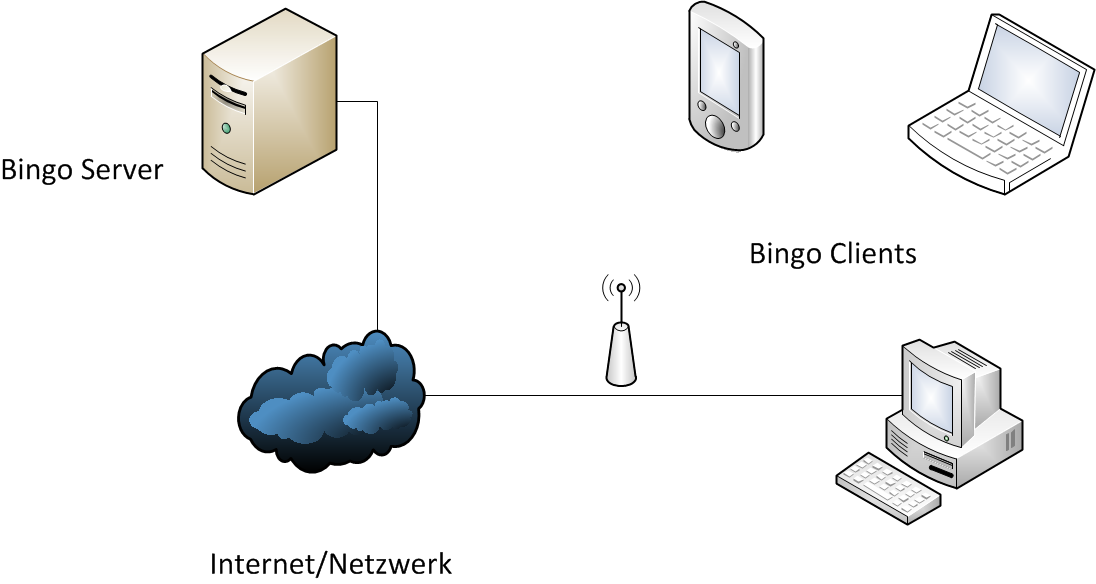
\includegraphics[height=4cm]{BingoClientServer.png}
\end{center}
\begin{itemize}
\item Klassisches Client/Server-Modell
\item Leicht zu implementieren
\item Im Bingo-Kontext sinniger als z.B. Peer-2-Peer
\end{itemize}
\end{frame}

\begin{frame}[fragile]
\frametitle{Spiel-Architektur, Persistenz}
\begin{itemize}
\item Jeder Spieler erhält ein "'Token"'
\begin{itemize}
\item Eine eindeutige ID
\item Wird beim ersten Login zum Nick gemappt
\item Verfällt nach 24 Stunden
\end{itemize}
\item BLAH BLAH
\end{itemize}
\end{frame}


\subsection{Kommunikation: HTTP \& JSON}
\begin{frame}[fragile]
\frametitle{Kommunikation: HTTP \& JSON}
\begin{itemize}
\item Protokoll: HTTP
\begin{itemize}
\item ASCII - leicht zu parsen
\item Implementierungen für (fast) jede Programmiersprache
\item Load-Balancing/Proxies möglich
\end{itemize}
\item Serialisierung: JSON
\begin{itemize}
\item JavaScript Object Notation
\item Leichtgewichtiger, textbasierter Datenaustausch
\item Eingebaute Datenstrukturen, u.a. Arrays, HashMaps, Strings, ...
\item Selbstdefiniertes Bingo-Protokoll: \\
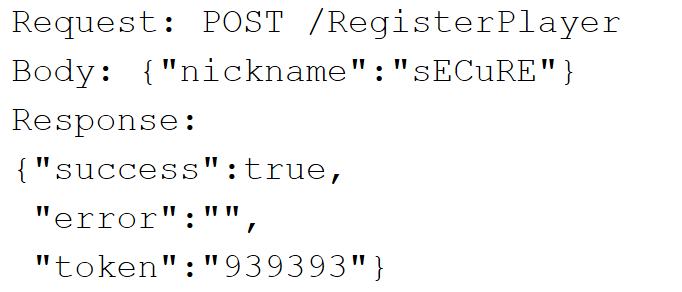
\includegraphics[height=2cm]{protocol.png}
\end{itemize}
\end{itemize}
\end{frame}

\section{Server}

\subsection{Perl}
\begin{frame}[fragile]
\frametitle{Server}
\begin{itemize}
\item Geschrieben in Perl
\item Test-Driven Development
\item Verwendete Module:
\begin{itemize}
\item Moose (Objektsystem für OOP)
\item Tatsumaki (Asynchrones Web-Framework)
\item JSON::XS (JSON En-/Decode)
\item Test::More (Test-Framework)
\end{itemize}
\end{itemize}
\end{frame}

\section{Clients}

\subsection{Qt-Client}
\begin{frame}[fragile]
\frametitle{Qt-Client - Eingesetzte Software}
\begin{itemize}
\item Qt
\begin{itemize}
\item GUI-Bibliothek für C++
\item Für alle gängigen Plattformen verfügbar
\item Viele Zusatzbibliotheken (z.B. QNetwork)
\end{itemize}
\item CMake
\begin{itemize}
\item = "'Cross-Platform Make"'
\item Eine Art Meta-Makefile
\item Ein Makefile für alle Plattformen
\end{itemize}
\item QJson
\begin{itemize}
\item JSON-Erweiterung für Qt
\item Serialisiert Klassen in Request-Daten
\item Liefert Antworten als abstrakten \texttt{QVariant} Datentypen
\end{itemize}
\end{itemize}
\end{frame}

\begin{frame}[fragile]
\frametitle{Qt-Client - Architektur}

\end{frame}

\begin{frame}[fragile]
\frametitle{Qt-Client - Demo}
Live demo?
\end{frame}

\subsection{Java-Client}
\begin{frame}[fragile]
\frametitle{Java-Client}
\begin{itemize}
\item GUI in Swing
\item JSON.org Java Implementierung
\item POST/GET via HTTPClient-Bibliothek der Apache Foundation
\end{itemize}
\end{frame}

\begin{frame}[fragile]
\frametitle{Java-Client - Architektur}
\begin{center}
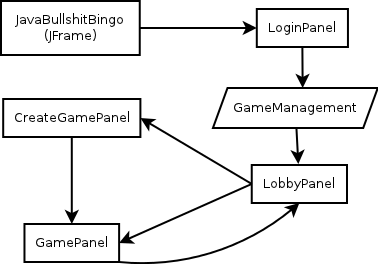
\includegraphics[height=4cm]{JBB_Aufbau.png}
\end{center}
\end{frame}

\subsection{Android-Client}

\begin{frame}[fragile]
\frametitle{Android-Client}
\begin{itemize}
\item Geschrieben in Mirah
\end{itemize}
\end{frame}

\begin{frame}[fragile]
\frametitle{Android-Client - Großes Geheimnis}
\begin{itemize}
\item Lüften des großen Geheimnisses
\end{itemize}
\end{frame}

\subsection{AJAX-Client}

\begin{frame}[fragile]
\frametitle{AJAX-basierte Web-Anwendung}
\begin{itemize}
\item Variante Nummer 4 :)
\item Basierend auf jQuery
\item JSON-Support durch jQuery gegeben
\item bbq-Plugin für Zustände (Token/Spiel-ID)
\end{itemize}
\end{frame}

\end{document}
